\documentclass[a4paper]{article}

\setlength{\parskip}{2mm}
\newcommand{\tab}{~ \qquad}

% paquetes
\usepackage{caratula} 
\usepackage{graphicx}
\usepackage{makeidx}
\usepackage{tocloft}
\usepackage{hyperref}
\hypersetup{
    colorlinks=true,     
    linkcolor=blue,     
    citecolor=blue,     
    urlcolor=blue        
}

\begin{document}

\titulo{Trabajo Práctico}
\subtitulo{Threading}
\fecha{22 de Octubre de 2024}
\materia{Sistemas Operativos}
\grupo{Grupo 11}

\newcommand{\dato}{\textit{Dato}}
\newcommand{\individuo}{\textit{Individuo}}

% Pongan cuantos integrantes quieran
\integrante{Valencia, Juan Segundo}{705/22}{juansegundovalencia@gmail.com}
\integrante{Melli, Tomás Felipe}{371/2}{tomas.melli1@gmail.com}
\integrante{Loria, Ezequiel}{111/16}{c03iff@hotmail.com}

\maketitle
\newpage

% índice
\renewcommand{\contentsname}{Índice}
\tableofcontents
\newpage


% INTRODUCCIÓN
\section{Introducción}\label{sec:intro}
\text{}
\newpage

% DESARROLLO
\section{Desarrollo}\label{sec:desarrollo}
\subsection{Operaciones Lista Atómica}\label{sec:op_lista_a}
\subsubsection{Insertar}\label{sec:insertar}

\text{En el primer ejercicio del TP nos piden completar el método insertar(T valor) de la clase ListaAtómica. Esta clase se utiliza para modelar una lista enlazada que se encargará de resolver las colisiones dentro del HashMap. Frente a muchas operaciones a la hora de querer agregar o incrementar elementos dentro de la lista, podría surgir que haya race condition, es decir, salidas que no correspondan a una serialización válida. Es por ello que se decide construir una lista que cumpla con la propiedad de atomicidad. Esta es la propiedad que tienen ciertas variables que al ser modificadas por alguna tarea, esta última no perderá el procesador durante su ejecución garantizando una correcta modificación de la misma. \\
Para cumplir con la propiedad de atomicidad, nuestra función insertar hace uso de la función compare exchange weak(expected , desired ) la cuál recibe como parametro el valor esperado de cabeza "el valor al cuál queremos enlazar al nuevo nodo" y el valor desired que es el nuevo nodo el cuál queremos que sea la nueva cabeza en la lista atómica. Para lograrlo la función en cada iteración verifica que el valor de nuevo.siguiente coincida con el desired (esta comparación es atómica y es weak por lo tanto podría ser desalojada) y en caso de devolver verdadero se efectua el cambio de cabeza. Por el otro lado, en caso de devolver false la función actualiza el valor de nuevo siguiente por el actual de cabeza (en el caso en que se inserte una nueva cabeza) y continua hasta que devuelva true y se inserte el nodo que queríamos insertar.  }
\\ \\
%imagen insertar l_atómica
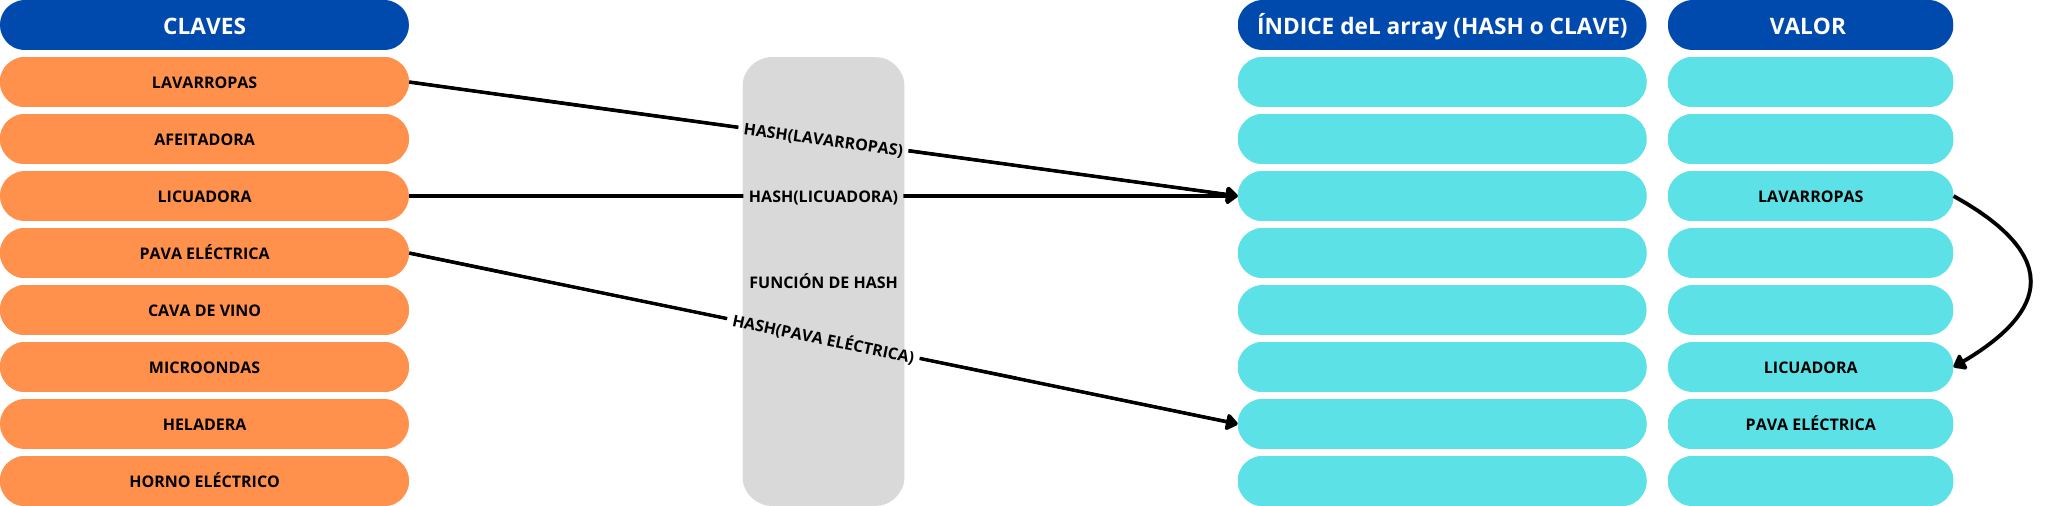
\includegraphics[width=1\textwidth]{ej1.png}
\newpage

\subsection{Operaciones Hash Map Concurrente}\label{sec:op_hm}
\subsubsection{Incrementar}\label{sec:Incrementar}
\text{En este ejercicio se nos pide implementar la función incrementar. Esta función recibe como paramétro una clave que deberá ser incrementada en caso de existir en la tabla, en caso de no existir, será agregada. Es evidente que se pueden dar condiciones de carrera cuando varios threads quieren modificar la misma lista (al existir una colision de hashes en la tabla). Para resolver esto se adopto el uso de semáforos binarios que garantizan un control sobre el acceso a la modificación de cada lista atómica. Dado que en la consigna se pide que sólo haya contención en caso de colisión de hash, optamos por no bloquear toda la tabla, sino sólamente la lista atómica correspondiente al hash reduciendo también el tiempo de espera de procesos que quieran ejecutar incrementar sobre otras claves que no colisionen entre sí.\\
}\\
%imagen incrementar
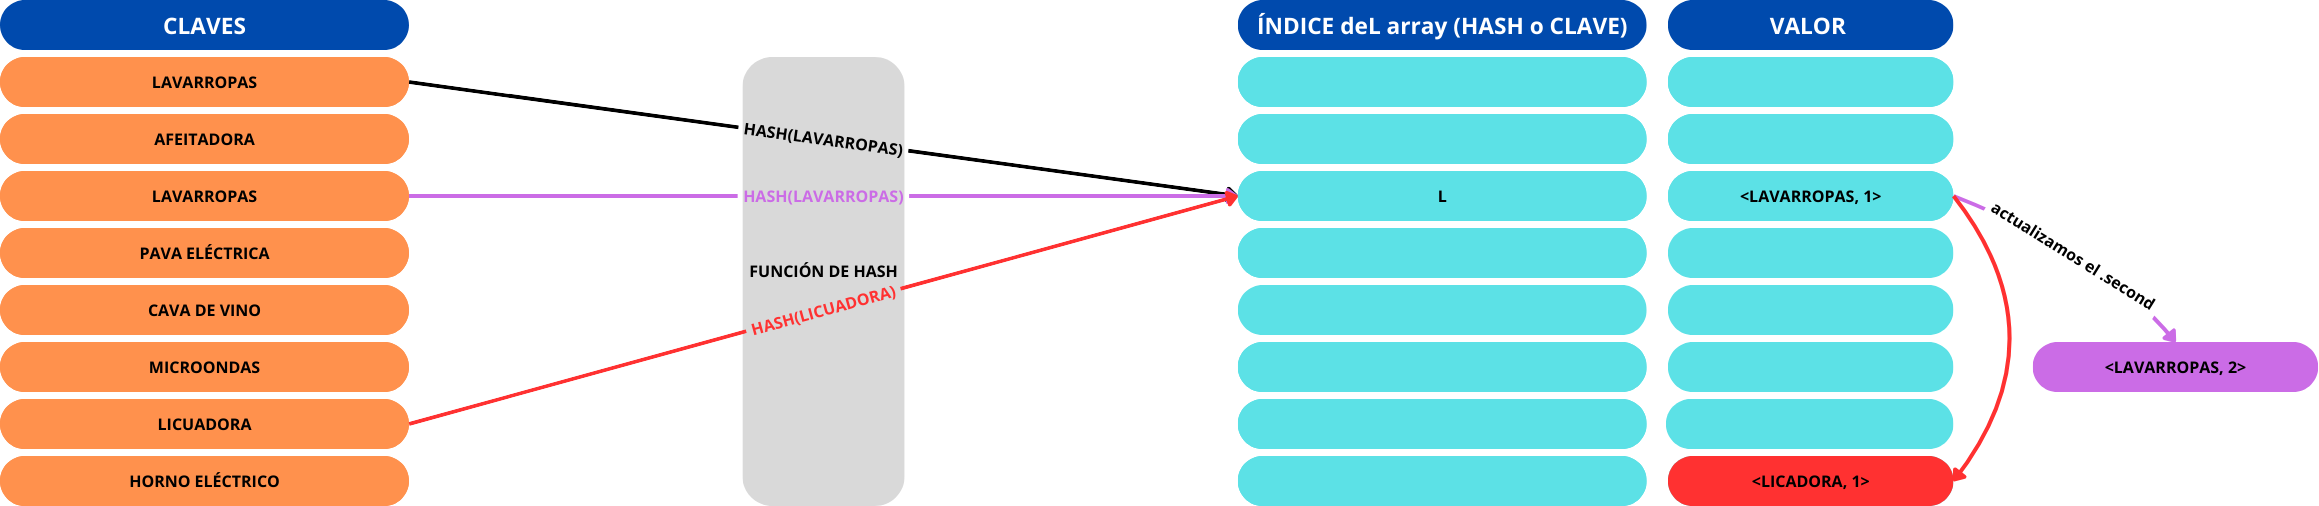
\includegraphics[width=1\textwidth]{ej2.png}

\subsubsection{Claves}\label{sec:Claves}
\text{La función claves devuelve un vector de todas las claves existentes en la tabla. Dado que en la consigna nos piden que sea no bloqueante y libre de inanición decidimos implementar esta función de manera que no se bloqueé toda la tabla por completo sino que únicamente la lista en la cuál se buscarán nuestras claves. Como consecuencia, si hay otros procesos intentando acceder a la tabla, solamente deberán esperar a que se libere la lista correspondiente.\\
**Durante la resolución del ejercicio tuvimos un debate sobre la consistencia del resultado de esta función. Dado que se podría dar la situación en que se agreguen claves en listas atómicas ya visitadas durante la ejecución de claves, al momento de retornar la función, los datos no serían exactamente los mismos que aquellos contenidos en la tabla en ese momento dado. Como respuesta a este problema se nos ocurrió bloquear toda la tabla, recorrer todas las listas y retornar todas las claves. Sin embargo esta forma de resolverlo no cumple con lo exigido en la consigna: NO BLOQUEANTE Y LIBRE DE INANICIÓN. Ya que bloquearía toda la tabla y en caso de tener muchos threads queriendo acceder a la tabla, se incurriría en largas esperas y como consecuencia en inanición. \\}

\subsubsection{Valor}\label{sec:Valor} 
\text{La función valor recibe como parametro una clave. La función deberá devolver el valor de dicha clave en la tabla si existe, sino 0. Como condición deberemos evitar que sea bloqueante y que haya inanición. Dicho esto, solamente estamos bloqueando la lista correspondiente a su hash y no toda la tabla. Esto garantizará que otros threads puedan acceder a la tabla (a excepción de la lista en la que sucede la búsqueda) sin incurrir en largas esperas. \\}

\subsubsection{Promedio}\label{sec:Promedio} 
\text{En el ejercicio 3 se pide devolver el promedio de la cantidad que tenemos de cierto producto. Esta operación requiere recorrer el HashMap en su totalidad. En el caso de querer ejecutar concurrentemente con incrementar, se podría dar el caso en que se quiera incrementar una clave en una lista de la cual promedio debe ir capturando los valores, generando cierta condición de carrera. En nuestra implementación, esto no sucede dado que incrementar deberá esperar a que se libere el mutex correspondiente a dicho hash. Sí podría suceder que se incremente una clave en una lista diferente a la que promedio está recorriendo, pero sólo en listas ya recorridas (dado que nosotros bloqueamos al inicio toda la tabla y luego se va liberando). Esto último garantiza que al momento de llamar a promedio() el valor de retorno sea consistente con el momento en el que se llamó. La idea de ir liberando garantiza que no haya tanto tiempo de espera por parte de incrementar. \\
Respecto al escenario mencionado en la consigna, nosotros logramos evitar modificaciones en listas aún recorridas y por tanto, un escenario de un resultado que no fue, no podría suceder. Sí podría suceder que el promedio devuelto no sea en el momento exacto en que retorna, pero se pide que incrementar pueda ejecutarse concurrentemente y por tanto no podremos bloquear completamente la tabla para garantizar dicha consistencia.\\}

\subsubsection{PromedioParalelo}\label{sec:PromedioParalelo} 
\text{En la función PromedioParalelo se buscará obtener el Promedio con la ayuda de distintos hilos de ejecución. La idea conceptual es definir una variable de tipo int atómica que defina en qué hash deberá buscar el thread lanzado. Esto garantiza que no haya dos threads buscando en la misma lista atómica y también que aquellos lanzados tendrán algo para hacer mientras tengan el proce en su poseción. Aquellos que lean un valor por fuera del rango de la tabla, terminarán su ejecución inmediatamente. Se define una función auxiliar en la que la tarea que deben cumplir es, capturar la cantidad total de elementos distintos y la cantidad total de elementos por lista asignada. Como valor de retorno, deberán insertar un par de enteros en el vector de pares que la función promedioParalelo procesará una vez que todos los threads hayan terminado de capturar la información anteriormente descripta. Los recursos que comparten los threads son : el hashmap, el vector de resultados y el atomic int.
Con la estrategia mencionada, no se modificó el tipo de dato que devuelve promedioParalelo pero sí se le exige recibir como parámetro cierta cantidad de threads para distribuir el trabajo.}\\
%imagen prom_paralelo
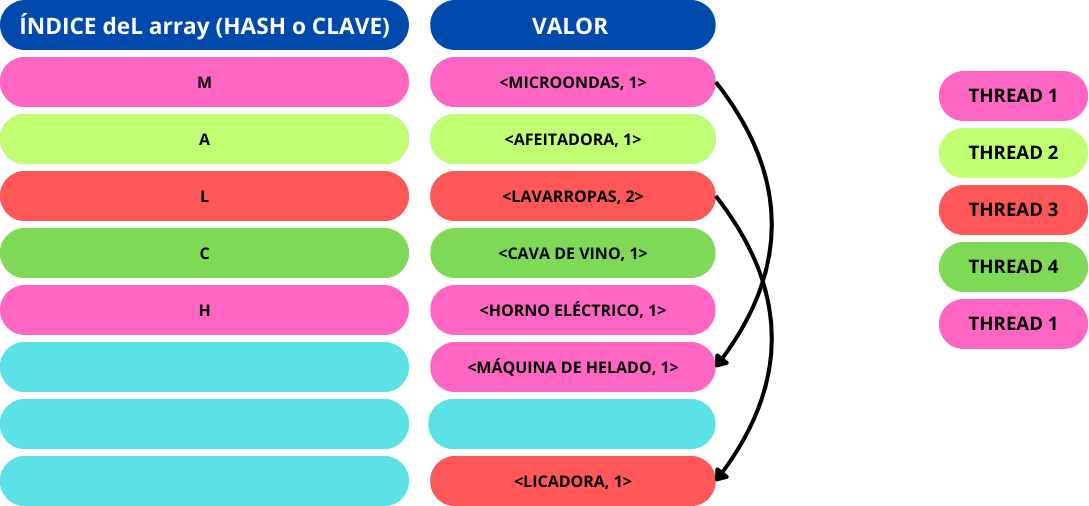
\includegraphics[width=0.7\textwidth]{ej3.png}

\section{Operaciones de Carga de Archivos}\label{sec:op_carga}
\subsubsection{Cargar Archivos}\label{sec:cargar_archivos} 

\text{En el ejercicio 4 se pide completar la implementación parcial de una función que dado un archivo carga en un hashmap los productos. Para completar la implementación simplemente hacemos uso de la función implementada en el ejercicio 2, incrementar. Como en esta función esta contemplada la concurrencia , el uso de la misma mantiene en nuestra funcion que no haya condiciones de carrera al cargar los productos del archivo. \\}
% imagen cargar
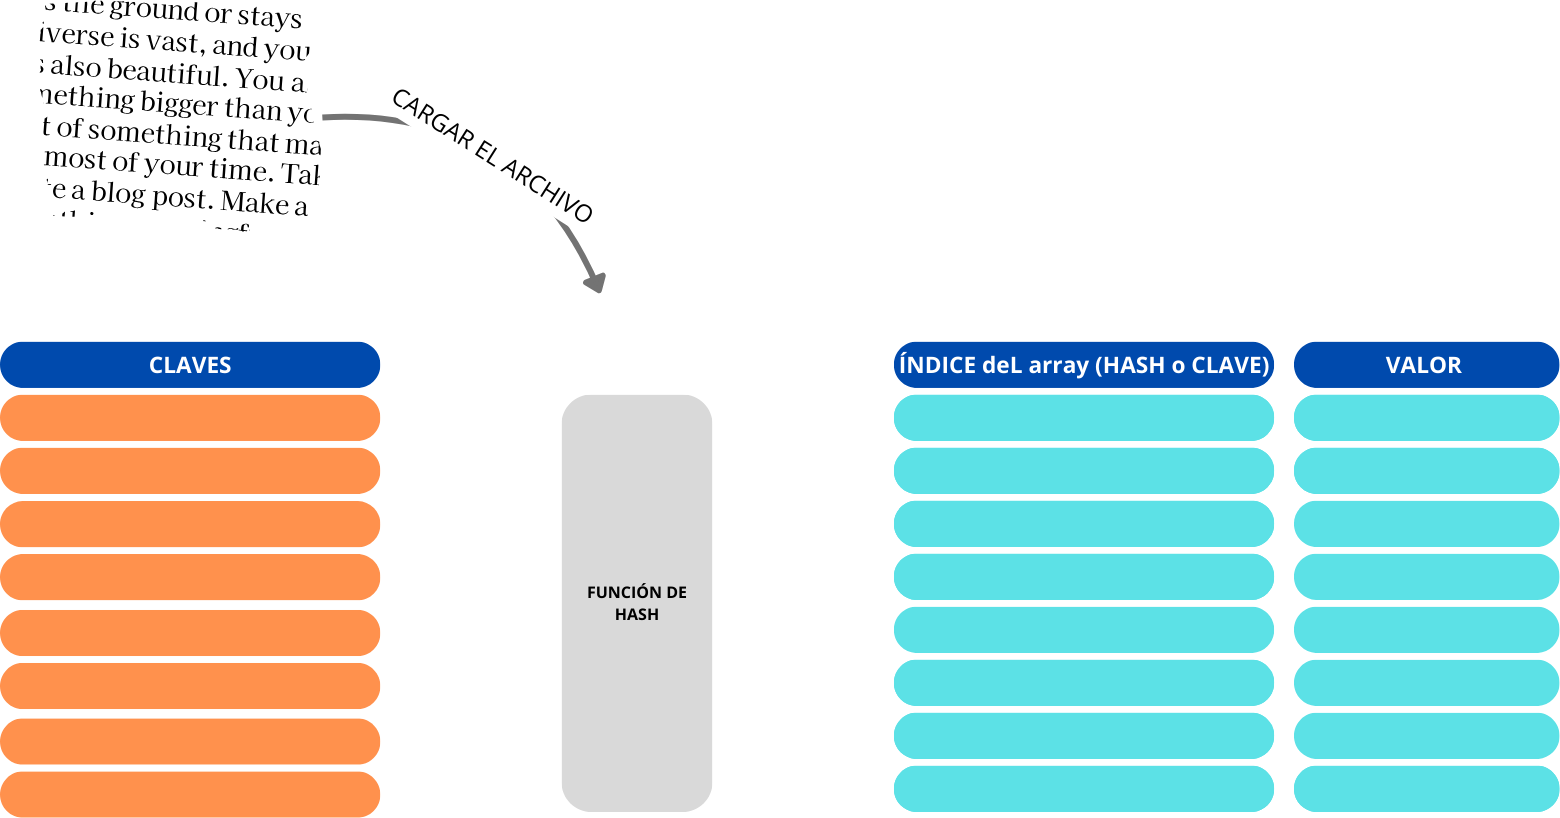
\includegraphics[width=0.7\textwidth]{ej4_a.png} 

\subsubsection{Cargar Múltiples Archivos}\label{sec:cargar_mult_archivos} 
\text{En el caso de la función cargar múltiples archivos, hacemos uso de una función auxiliar cargar que ejecutaran nuestros threads en la que se le de adjudicara un archivo a cada uno siempre que haya archivos disponibles. Para asegurar que no haya dos threads cargando el mismo archivo hacemos uso de la variable atómica archivo que denotara el archivo a cargar.\\ \\}
%imagen  cargar_mult
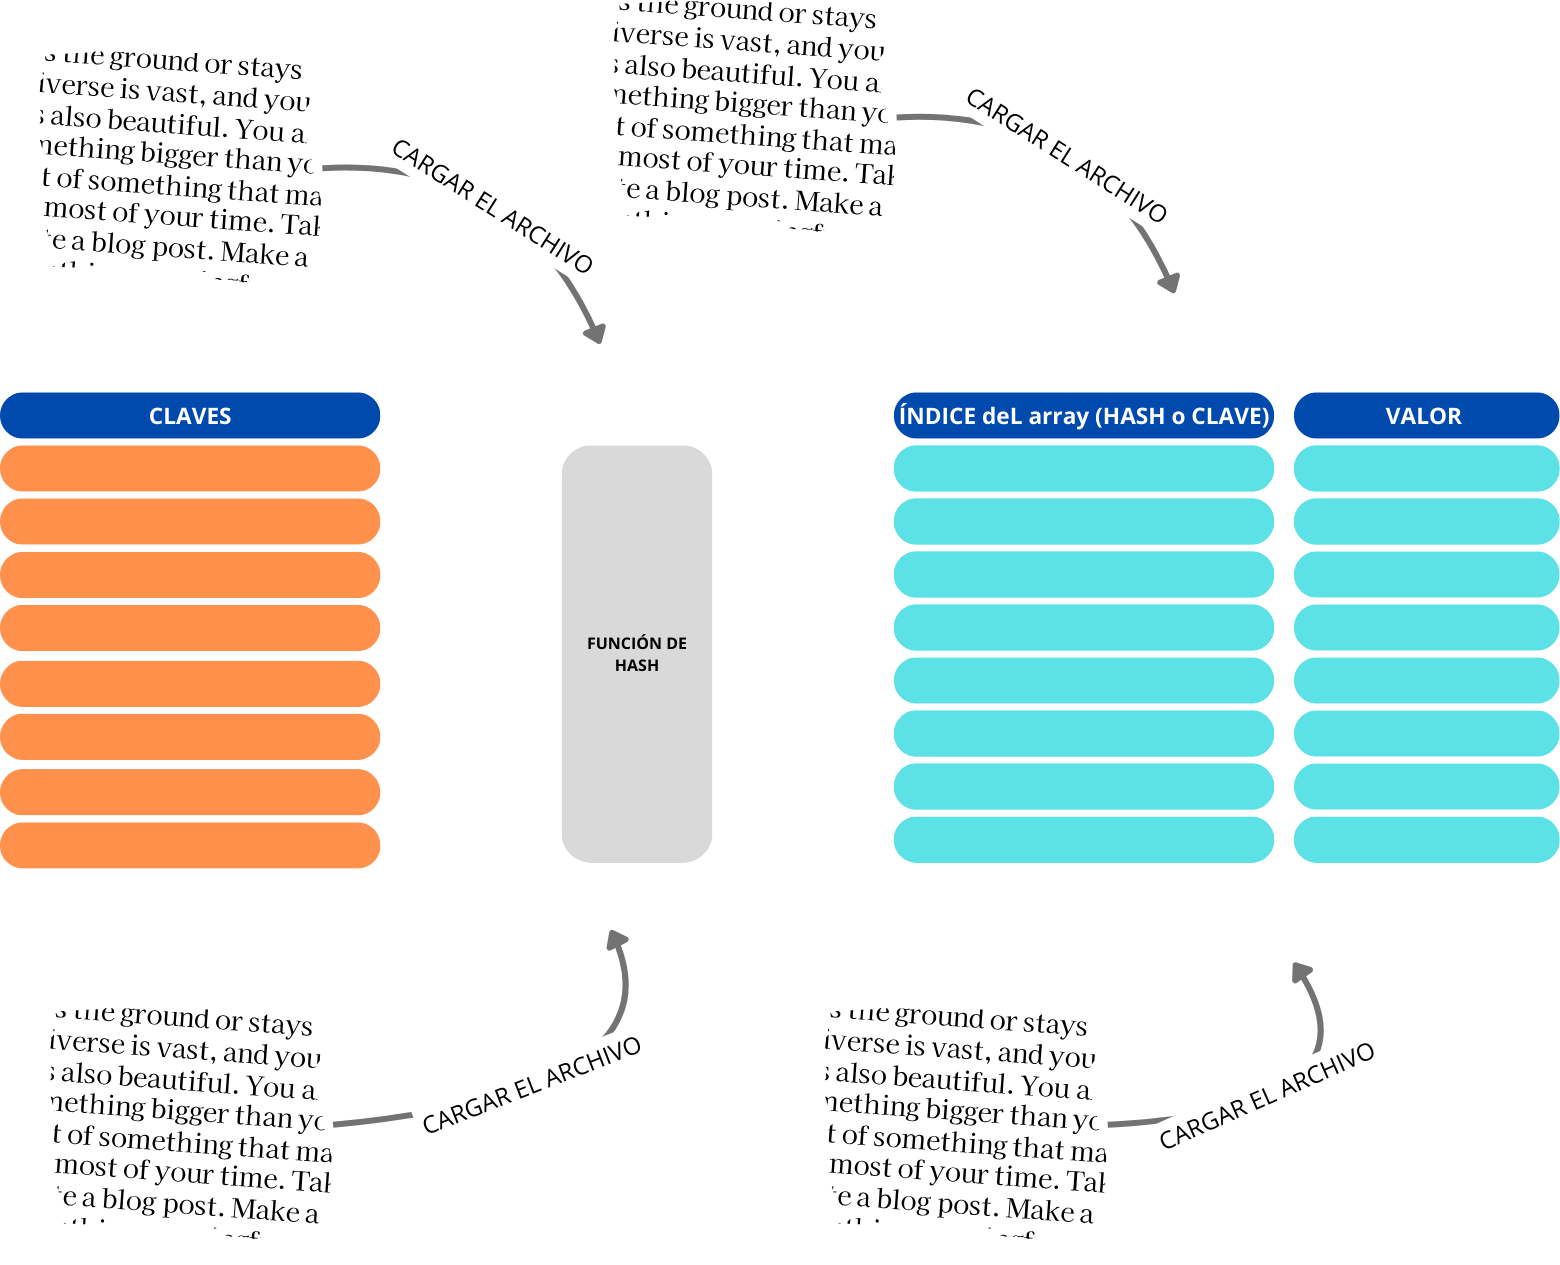
\includegraphics[width=0.7\textwidth]{ej4.png}

\section{Últimas consideraciones}\label{sec:consideraciones}
\text{En el contexto de un black friday donde se reciben millones de compras y la cantidad de productos sufre modificaciones constantemente se deberá garantizar que el comprador de producto disponga de su producto. Problemas de consistencia generaria ventas sin stock, con este sistema ya vimos que la función incrementar/decrementar a pesar de ejecutarse muchas veces no se perderá información. Sin embargo se podría incurrir en cierta espera. De todos modos estamos satisfechos con nuestra implementación.\\
Tuvimos en consideración la posibilidad de implementar un mutex para cada producto de manera de no bloquear toda la lista atómica. Dado que la cantidad de hashes es baja y la cantidad de colisiones será muy alta. \\
En el contexto de una tienda que vende sólo dos productos la concurrecia es vital al momento de que lleguen pedidos de compra o de incremento del stock. Por tanto, la contención será más pronunciada. Es vital implementar un modelo que evite race condition.\\
En el caso de querer implementar la función calcularMedianaParalela, se optaría por implementar un algoritmo de sorting en el que cierta cantidad de threads tomarían la labor de ordenar los valores. Es decir, se capturarían todos los datos en un vector compartido, en el que los threads pushearían los valores y luego cada uno tomaría cierta partición para realizar el ordenamiento. MergeSortParalelo para el ordenamiento y finalmente, mirar el dato medio del vector ordenado ( en caso de ser par, sorted[medio - 1] + sorted[medio] / 2). 
}

\section{Tests}\label{sec:Tests}
\subsection{Test : PromedioParalelo}\label{sec:test_pp}

\section{Conclusiones}\label{sec:Conclusiones}
\end{document}
